\documentclass[12pt]{article}
\usepackage[utf8]{inputenc}
\usepackage[english]{babel}

\usepackage[style=IEEE]{biblatex}
\addbibresource{Bibliography.bib}

\usepackage{siunitx}
\usepackage{fullpage}
\usepackage{amsmath, amssymb}
\usepackage{enumerate}
\usepackage{mathtools}
\usepackage{amsthm}
\usepackage{graphicx}
\usepackage{listings}
\usepackage{color}
\usepackage{verbatim}
\usepackage{float}
\usepackage[table]{xcolor}
\restylefloat{table}
\usepackage[parfill]{parskip}
\usepackage{xcolor}
\usepackage{caption}
\usepackage{subcaption}
\usepackage{multicol}
\usepackage{blindtext}
\usepackage{paracol}
\usepackage{tabularx}
\usepackage{ragged2e}
\usepackage{multirow}
\usepackage{multicol}
\usepackage{pdflscape}
\usepackage{chngpage}


\newcolumntype{M}[1]{>{\centering\arraybackslash}m{#1}}


\usepackage{tikz}
\usetikzlibrary{shapes.geometric, arrows}
\tikzstyle{startstop} = [rectangle, rounded corners, minimum width=3cm, minimum height=1cm,text centered, draw=black, fill=red!30]
\tikzstyle{io} = [trapezium, trapezium left angle=70, trapezium right angle=110, minimum width=3cm, minimum height=1cm, text centered, draw=black, fill=blue!30]
\tikzstyle{process} = [rectangle, minimum width=3cm, minimum height=1cm, text centered, draw=black]
\tikzstyle{decision} = [diamond, minimum width=3cm, minimum height=1cm, text centered, draw=black, fill=green!30]
\tikzstyle{arrow} = [thick,->,>=stealth]


\definecolor{codegreen}{rgb}{0,0.6,0}
\definecolor{codegray}{rgb}{0.5,0.5,0.5}
\definecolor{codepurple}{rgb}{0.58,0,0.82}
\definecolor{backcolour}{rgb}{0.95,0.95,0.92}

\lstset{ 
	language=Matlab,
%	basicstyle=10pt,
	numbers=left,
	stepnumber=1,
	numbersep=5pt,
%	backgroundcolor=\color{white},  	% choose the background color. You must add \usepackage{color}
	showspaces=false,
	showstringspaces=false,
	showtabs=false,
%	frame=single,
%	tabsize=2,
%	captionpos=b,
	breaklines=true,
	breakatwhitespace=false,
	backgroundcolor=\color{backcolour},   
    commentstyle=\color{codegreen},
    keywordstyle=\color{blue},
    numberstyle=\footnotesize\color{codegray},
    stringstyle=\color{codepurple},
	escapeinside={\%*}{*)}
}
\tolerance=1
\emergencystretch=\maxdimen
\hyphenpenalty=10000
\hbadness=10000
\begin{document}

\begin{titlepage}
	\centering
	\vspace{1cm}
	{\scshape\LARGE The University of Queensland \par}
	\vspace{1cm}
	{\scshape\Large ENGG4802\par}
	\vspace{1.5cm}
	{\huge\bfseries Project Proposal \par}
	\vspace{2cm}
	{\Large\scshape Anna Nguyen 44317300\par}
	\vfill
	Supervised by\par
	Dr. Richard \textsc{Yan}

	\vfill

% Bottom of the page
	{\large 03 September, 2020\par}
\end{titlepage}

\tableofcontents

\newpage
\section{Topic Definition}
\subsection{Motivation}
Power systems are integral in the supply and distribution of electricity for use in all facets of society. As a result, it is important to quickly detect and classify any faults in order to prevent catastrophic and potentially permanent failures. Although there are already many pieces of fail-safe equipment and systems put in place to  control the severity of a potential fault, real-time event detection and classification is extremely important in gaining insight to the nature and cause of a fault. \newline 
\\
Given that a power system has many sub-systems which all have specific purposes, there are many areas where faults can occur. These can range from equipment failures, such as regular deterioration over time or faulty parts, to faults due to the external environment, such as lightning strikes or tree branches brushing up against transmission lines, all of which will produce a certain disturbance signature in the waveform of the power system. \newline 
\\
If undetected, faults in a power system are signs of and can lead to permanent failures in the system. One consequence of a permanent failure is power outages in downstream services, which would be detrimental to society if such services are essential. However, a failure can also result in the the breakdown of multiple components that make up a power system whose recommissioning and replacement can be time consuming and extremely costly. 

Energy distributors and retailers have an obligation and responsibility to provide energy to consumers at determined standards. When these standards are not met, distributors are required to make guaranteed service level (GSL) payments to consumers, whose value depends on the type of interruption and its frequency and duration. \newline
\\ 
For the 2018-19 financial year, the Queensland Competition Authority (QCA) reported that Ergon Energy and Energex paid \$1.2 million and \$3.4 million in GSL payments respectively \cite{QCA}. From this value, 94.6\% and 93.6\% of the respective payments came from reliability interruptions. Consequently, being able to detect and recognise the cause of an interruption will potentially reduce costs to distribution companies, but also reduce the duration of faults, resulting in higher reliability for consumers.



\newpage
\subsection{Project Outline}
The proposed project is the automatic detection of events in a power system caused by faults with data provided by power quality meters. In addition to this, the classification of a detected fault will also be considered. This is due to the many types of faults (steady-state, transient, intermittent) caused by various events and resulting in varying severity as a consequence. A successful automatic detection and classification of a fault and its cause is extremely beneficial to power systems management as it prevents catastrophic failures and costly replacement of equipment as well as reducing the time taken to  determine the cause of the fault.
\subsubsection{Objectives}
Data will be collected from a power quality meter connected to an aged transformer located in a substation at the University of Queensland St Lucia campus. A successful project details the reading and analysis of large amounts of data from the meter which results in a reliable high rate of detection any events. There are currently many algorithms being implemented to automatically detect events in power system waveforms - including digital signal processing methods and neural networks. These methods differ and as a result, will have certain advantages and disadvantages compared with each other. A decision making criteria will be created in order to determine the most successful algorithm(s) and will be chosen for the final demonstration. The majority of the programming and computation will be completed with Python.\newline
\\
After a high rate of detection is achieved, the fault is then classified into one of three main disturbance categories: Steady-state, Transient or Intermittent. Within these subsections, the specific type of fault will be classified from analysing and researching waveform signatures of known disturbances. A detected fault will be classified using the standards and indices as defined by the the Institute of Electrical and Electronics Engineers (IEEE) Std. 1159-2009 \cite{PQ}.   

Depending on its cause, some faults may be self-clearing and never occur again. However, some of these self-clearing faults are incipient to permanent failures which will require the operation of protective devices such as breakers. As a result, it is extremely important to classify not only the type of power system fault, but also whether such fault will result in costly permanent failures. Analysis and research into various causes of faults will be conducted in order to further define and classify the consequence of any particular power system event. 



\newpage 
\section{Background}
\subsection{Power Quality Disturbances} 
A non-disturbed power system should supply three-phase AC (sinusoidal) voltage and current to consumers. When faults in the system occur, we can see interference in one or more of the provided waveforms. Power Quality disturbances are separated into three main categories as characterised by IEEE 1159-2019\cite{PQ}.

{\renewcommand{\arraystretch}{1.2}	
\begin{table}[h!]
\centering
\noindent
\begin{tabular}{|>{\RaggedRight}p{0.2\textwidth}|p{0.4\textwidth}|p{0.4\textwidth}|}
\hline
Disturbance Type & Characteristics & Potential Causes and Consequences \\
\hline
\textbf{\underline{Steady-state}}  &  \textbf{\underline{$>$ 1 min}} & \\
\hline
Over-voltages \& Under-voltages &  One or more phases of voltage is higher than 1.1pu or lower than 0.9pu.& Load variations or system switching.\\
Sustained Interruptions & Supply voltage is reduced to less than 0.1pu. & Typically permanent - will require operation of protective devices or manual intervention.\\
Voltage \& Current Imbalances & Refers to the ratio between the magnitudes of negative and positive sequence components of a three phase system. & Commonly occurs when multiple single phase loads are unbalanced on a three phase system.\\
\hline
\textbf{\underline{Transient}}  &  \textbf{\underline{$<$ 1 min}} & \\
\hline
Voltage sags \& swells & One or more phases of voltage is higher than 1.1pu or lower than 0.9pu.& High starting currents from load energisation/switching or faulty physical connections/equipment.\\
Interruptions & Supply voltage is reduced to less than 0.1pu.& Faulty equipment, power systems faults.\\
Impulsive transients & Sudden, large and unidirectional changes in a waveform. & Lightning Strikes.\\
Oscillatory transients & Waveforms exhibit a rapid increase in frequency, changing polarity with each period before the disturbance clears. & Capacitor/cable switching.\\
Frequency variation & Deviation from the fundamental frequency. & Imbalance between load and generator capacity.\\
\hline
\textbf{\underline{Intermittent}}  & \textbf{\underline{$<$ 25 Hz}} & \\
\hline 
Flickering & Small fluctuations in the voltage waveform.& Arcing, loads with reactive cyclic variations.\\
\hline
\end{tabular}
\caption{Disturbance Types \& Characteristics}
\end{table}


\newpage
\subsection{Existing Event Detection Methods}
\subsubsection{Waveform Abnormality Methods}





There are many types of waveform abnormality detection methods, but the general method is:
\begin{enumerate}
\item Calculate the differential waveform between two periods
\item Determine if the differential waveform exceeds a certain threshold for a disturbance to have occurred
\end{enumerate}
For some chosen threshold, varieties of this method can include:

\begin{table}[H]
\centering
\begin{tabular}{|>{\RaggedRight}p{0.3\textwidth}|>{\RaggedRight}p{0.3\textwidth}|>{\RaggedRight}p{0.3\textwidth}|}
\hline
Description & Disturbance Criteria & Notes\\
\hline
The difference of two consecutive cycles calculated for each sample & Magnitude and duration of disturbance & Choosing a meaningful threshold value can be difficult\\
\hline
The difference of the square of two consecutive cycles calculated for each sample & Absolute value of difference & Squaring a sample not technically sound and can remove some sensitivities\\
\hline
RMS of the difference of two consecutive cycles calculated & Percentage difference between 'healthy' RMS value & Considers the RMS value of a whole cycle and disturbances which last less than a cycle may not be detected\\
\hline
\end{tabular}
\caption{Waveform Detection Method Variations}
\end{table}

The above methods are computationally simple, but have drawbacks in the choosing of thresholds and detection sensitivity. Furthermore, choosing two consecutive cycles may not detect steady-state events such as over- and under-voltages. \newline
\\
A hypothesis test based detection method is detailed by Li et al. \cite{WA} by considering the expected random noise of a (current) waveform. Consider two hypotheses, $H_0$ being the waveform of a power system under normal operation and $H_1$ being the waveform of a power system under abnormal operation:
$$H_0: i(t) = \sum^K_{k=0}A_k\cos(2\pi k f_r t + \phi_k) + n(t)$$
$$H_1: i(t) = \sum^K_{k=0}A_k\cos(2\pi k f_r t + \phi_k) + n(t) + a(t)$$
where:
\begin{align*}
n(t) &\rightarrow \quad \text{Random noise}\\
a(t) &\rightarrow \quad \text{Abnormal component}\\
A_k\cos(2\pi k f_r t + \phi_k) &\rightarrow \quad \text{Steady state component}
\end{align*}

Removing the steady state component for abnormality detection:
\begin{align*}
H_0: i(t) &= n(t)\\
H_1: i(t) &= n(t) + a(t)
\end{align*}
It can be seen that under normal operation, only random noise should be left and under abnormal operation, there is superposition of random noise and an abnormal component. Differential waveforms that contain noise that doesn't resemble a normal distribution (Gaussian) is considered to be abnormal and contain an event.

\begin{figure}[H]
\centering
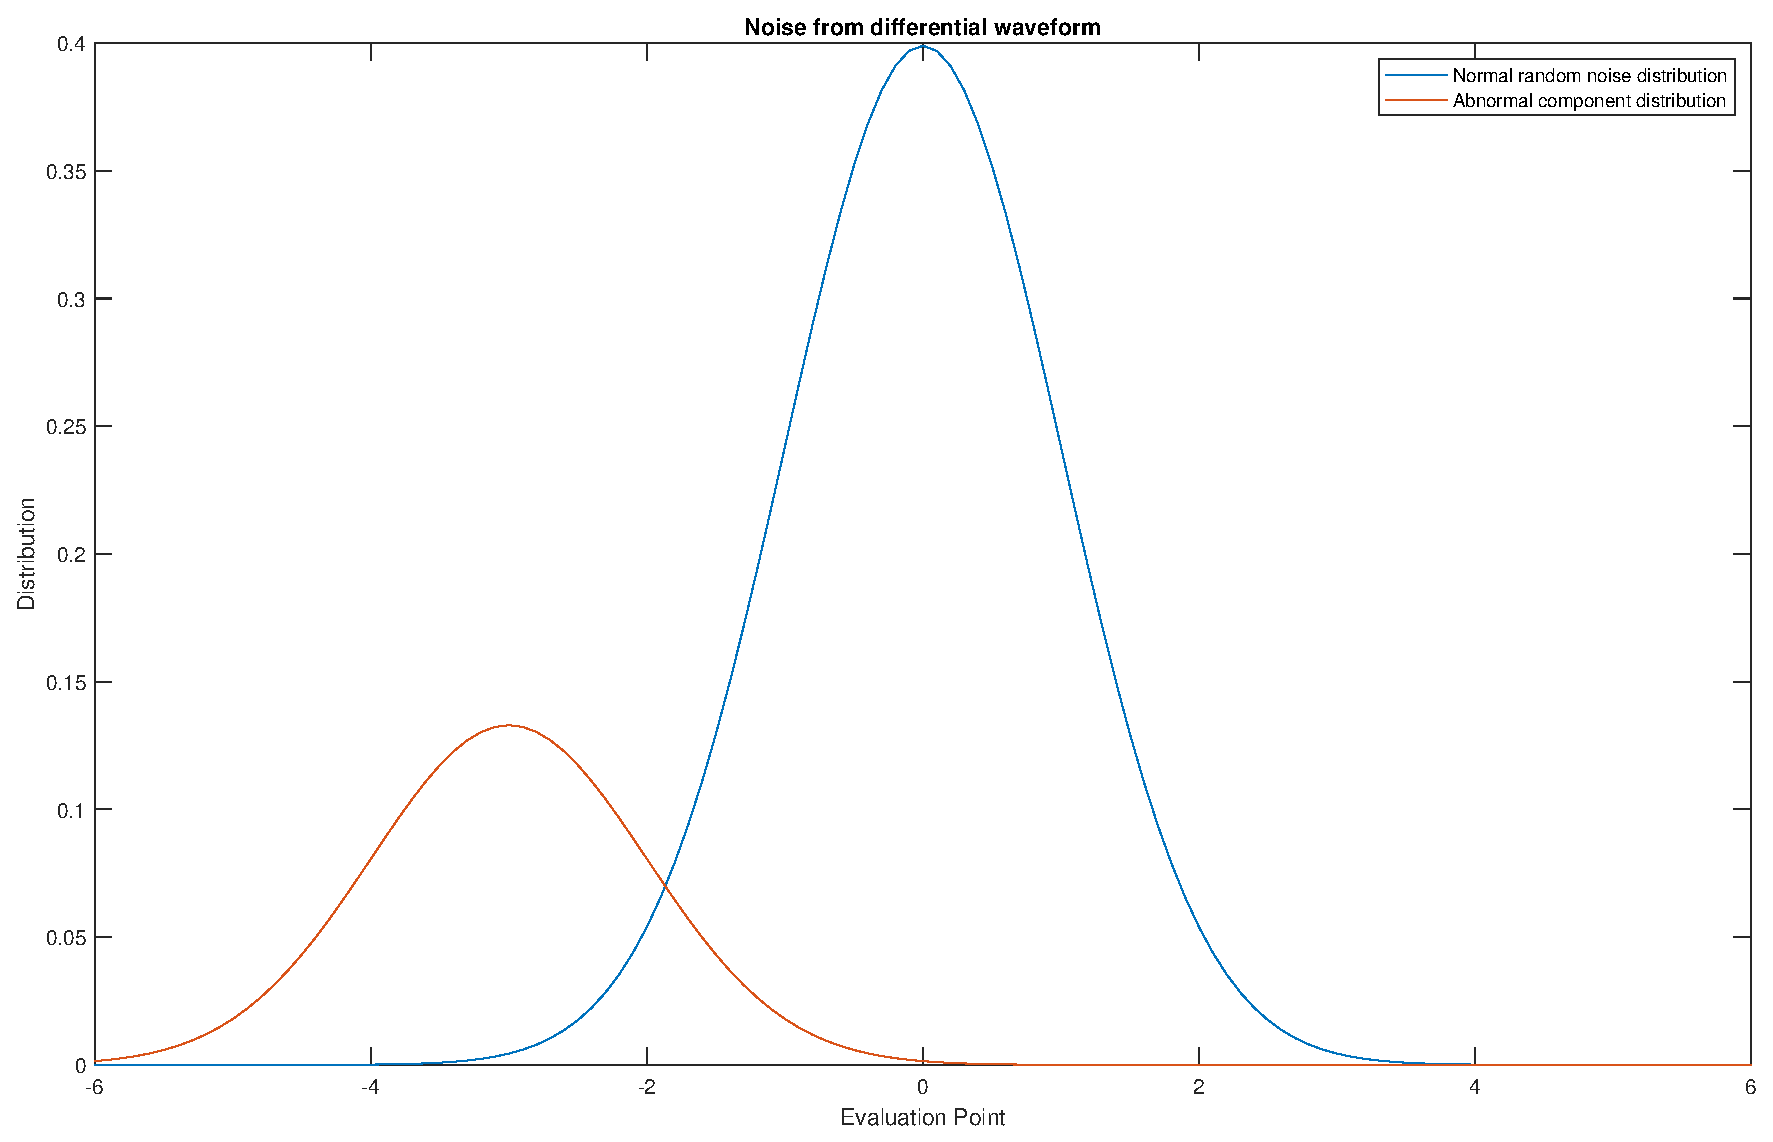
\includegraphics[scale=0.45]{WAH}
\caption{Expected random noise distribution (blue) vs. abnormal noise distribution (red) }
\end{figure}


\newpage
\subsubsection{Wavelet Analysis}
The wavelet analysis is often used to detect transient faults by  transforming a waveform into its frequency domain using the Fourier Transform. This is then decomposed into multiple approximations of the signal using various digital signal processing methods until sufficient bands of frequency ranges have been extracted (including the fundamental frequency).

\begin{figure}[H]
\centering

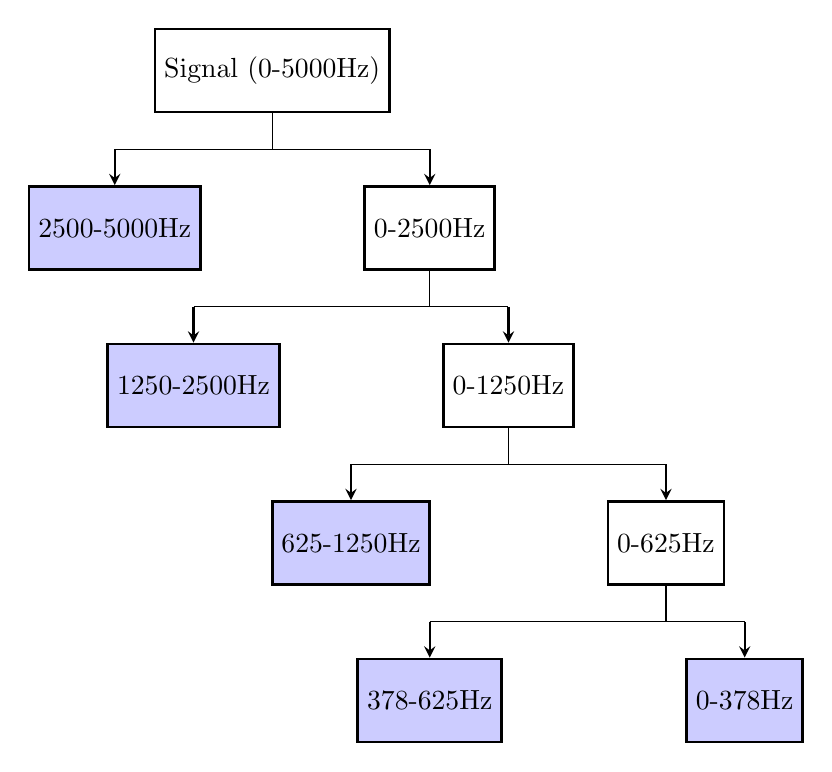
\begin{tikzpicture}[node distance=1cm]
    \tikzset{final/.style = {draw, shape=rectangle, minimum height=3em, minimum width=3em, node distance=2cm, line width=1pt, fill = blue!20},
    process/.style = {draw, shape=rectangle, minimum height=3em, minimum width=3em, node distance=2cm, line width=1pt},
     sum/.style = {draw, shape=circle, node distance=1.5cm, line width=1pt, minimum width=1.25em}, connection/.style={inner sep=0,outer sep=0}}

\node (signal) [process] {Signal (0-5000Hz)};
\coordinate [below of=signal] (cont) {};
\draw (signal) -- (cont);
\coordinate [below of=cont] (cont) {};
\node (upper) [final, left of=cont] {2500-5000Hz};
\node (lower) [process, right of=cont] {0-2500Hz};
\coordinate [above of = upper] (ajoint);
\coordinate [above of = lower] (bjoint);
\draw (ajoint) -- (bjoint);
\draw [arrow] (ajoint) -- (upper);
\draw [arrow] (bjoint) -- (lower);

\coordinate [below of = lower](cont) {};
\draw (lower) -- (cont);
\coordinate [below of=cont] (cont) {};
\coordinate [left of=cont] (cont) {};
\node (upper) [final, left of=cont] {1250-2500Hz};
\node (Lower) [process, right of=cont] {0-1250Hz};
\coordinate [above of = upper] (ajoint);
\coordinate [above of = Lower] (bjoint);
\draw (ajoint) -- (bjoint);
\draw [arrow] (ajoint) -- (upper);
\draw [arrow] (bjoint) -- (Lower);
\coordinate [below of = Lower](cont) {};
\draw (Lower) -- (cont);
\coordinate [below of=cont] (cont) {};

\coordinate [left of=cont] (conta) {};
\node (upper) [final, left of=cont] {625-1250Hz};
\node (Lower) [process, right of=cont] {0-625Hz};
\coordinate [above of = upper] (ajoint);
\coordinate [above of = Lower] (bjoint);
\draw (ajoint) -- (bjoint);
\draw [arrow] (ajoint) -- (upper);
\draw [arrow] (bjoint) -- (Lower);
\coordinate [below of = Lower](cont) {};
\draw (Lower) -- (cont);
\coordinate [below of=cont] (cont) {};

\coordinate [left of=cont] (cont) {};
\node (upper) [final, left of=cont] {378-625Hz};
\node (Lower) [final, right of=cont] {0-378Hz};
\coordinate [above of = upper] (ajoint);
\coordinate [above of = Lower] (bjoint);
\draw (ajoint) -- (bjoint);
\draw [arrow] (ajoint) -- (upper);
\draw [arrow] (bjoint) -- (Lower);

\end{tikzpicture}
\caption{Example decomposition of 5000Hz signal with chosen frequency bands in blue}
\end{figure}

Once the decompositions have been completed to satisfactory ranges, a disturbance is deemed to be detected if the magnitude in the decomposition exceeds a specified magnitude. We also note that disturbances in the high frequency detail typically occur from transient faults. \newline
\\
Detection based on these approximations are defined in \cite{PES} through the following equations. 
For decompositions on or near the fundamental frequency, a disturbance is detected for some threshold $\epsilon$ if:
$$RMSCR = \frac{RMS_{\text{latest half cycle}} - RMS_{\text{one cycle before}}}{RMS_{\text{one cycle before}}} > \epsilon$$
For decompositions of higher frequency, a disturbance is detected for some threshold $\epsilon$ if:
$$ENGR = \frac{\text{Energy}_{\text{latest}} - MEAN(\text{Energy}_{\text{past}})}{STD(\text{Energy}_\text{past})} > \epsilon$$

Additionally, the patent by Mousavi et al. \cite{FFC} discusses methods in determining events from the fundamental frequency approximation:
\begin{enumerate}
\item Complete DFT for $\frac{1}{2}$ a period of an input signal every $\frac{1}{8}^{th}$ cycle
\item Determining the threshold:
\begin{itemize}
\item Fixed
\item Dynamic
\end{itemize}
\end{enumerate}

Methods such as the S-Transform and the Fourier Transform and its variations (discrete (DFT), short-time (STFT)) are similar in its methods in that an input signal is decomposed into its spectrum components.\\
\\
The wavelet transform's advantages lie in the decomposition of the waveform, allowing for the detection of both transient and steady-state disturbances, whereas other methods such as waveform analysis may only detect transient faults. 

\newpage
\subsubsection{Artificial Neural Networks (Adaline)}
Artificial neural networks (ANN) look to mimic biological neural networks in the brain by 'learning' to classify certain input data. ANNs are commonly used for modelling and prediction for a multitude of applications. The general structure for an ANN is:
\begin{itemize}
\item Input Layer
\item Hidden Layer(s)
\item Output Layer
\end{itemize}

The hidden layers are composed of specific weights and functions which are programmed by training the network: a recursive method where inputs with known outputs are fed into the system. The desired and actual outputs are compared and any errors are propagated back into the hidden layers so their weights and functions can be altered until the output is achieved.

Adaptive Linear Neuron (Adaline) is a single layer neural network which takes in time delayed samples of the power system waveform and predicts the future waveform.\\


\begin{figure}[H]
\centering
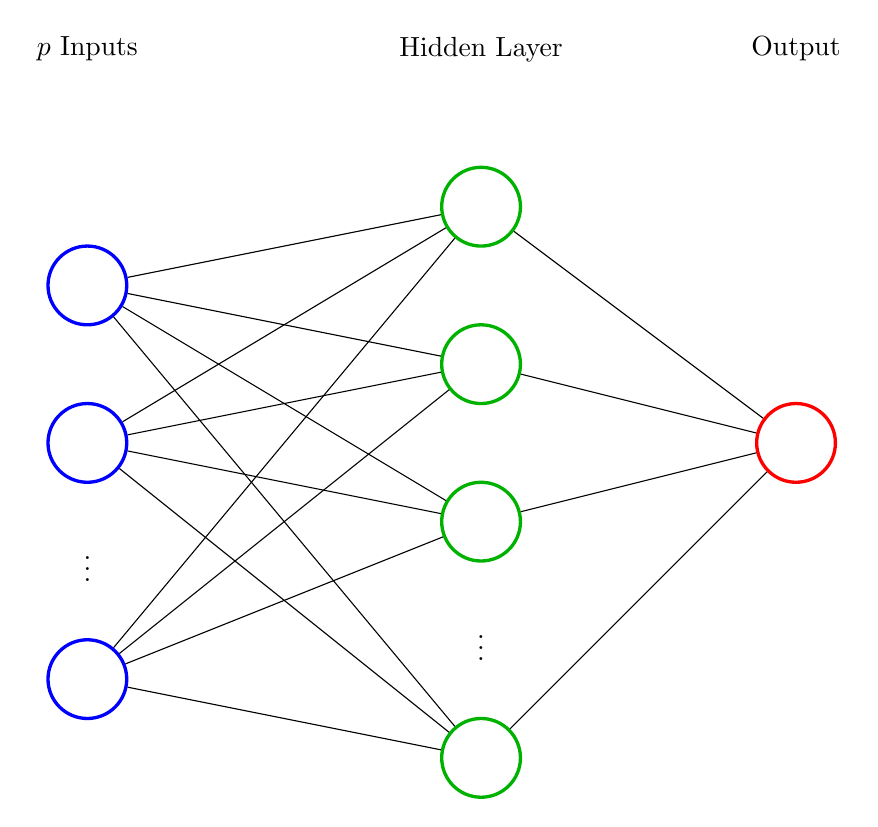
\begin{tikzpicture}[node distance=1cm, 
inputnode/.style={circle, draw=blue, very thick, minimum size=10mm},
hiddennode/.style={circle, draw=black!30!green, very thick, minimum size=10mm},
outputnode/.style={circle, draw=red, very thick, minimum size=10mm},]
\node[inputnode](input1){};
\coordinate [below of=input1] (cont) {};
\node[inputnode, below of = cont](input2){};
\coordinate [below of=input2] (cont) {};
\coordinate [below of=cont] (cont) {};
\node[inputnode, below of = cont](input3){};
\coordinate [right of=input1] (cont) {};
\coordinate [right of=cont] (cont) {};
\coordinate [right of=cont] (cont) {};
\coordinate [right of=cont] (cont) {};
\coordinate [right of=cont] (cont) {};
\node[hiddennode, above of = cont](hidden1){};
\coordinate [below of=hidden1] (cont) {};
\node[hiddennode, below of = cont](hidden2){};
\coordinate [below of=hidden2] (cont) {};
\node[hiddennode, below of = cont](hidden3){};
\coordinate [below of=hidden3] (cont) {};
\coordinate [below of=cont] (cont) {};
\node[hiddennode, below of = cont](hidden4){};
\coordinate [right of=input2] (cont) {};
\coordinate [right of=cont] (cont) {};
\coordinate [right of=cont] (cont) {};
\coordinate [right of=cont] (cont) {};
\coordinate [right of=cont] (cont) {};
\coordinate [right of=cont] (cont) {};
\coordinate [right of=cont] (cont) {};
\coordinate [right of=cont] (cont) {};
\node[outputnode, right of = cont](output){};
\path (input2) -- node[auto=false]{\vdots} (input3);
\path (hidden3) -- node[auto=false]{\vdots} (hidden4);
\draw (input1) -- (hidden1);
\draw (input1) -- (hidden2);
\draw (input1) -- (hidden3);
\draw (input1) -- (hidden4);
\draw (input2) -- (hidden1);
\draw (input2) -- (hidden2);
\draw (input2) -- (hidden3);
\draw (input2) -- (hidden4);
\draw (input3) -- (hidden1);
\draw (input3) -- (hidden2);
\draw (input3) -- (hidden3);
\draw (input3) -- (hidden4);
\draw (hidden1) -- (output);
\draw (hidden2) -- (output);
\draw (hidden3) -- (output);
\draw (hidden4) -- (output);
\coordinate [above of=input1] (cont) {};
\coordinate [above of=cont] (cont) {};
\node[above of = cont](inputtxt) {$p$ Inputs};
\coordinate [right of=inputtxt] (cont) {};
\coordinate [right of=cont] (cont) {};
\coordinate [right of=cont] (cont) {};
\coordinate [right of=cont] (cont) {};
\node[right of = cont](hiddentxt) {Hidden Layer};
\coordinate [right of=hiddentxt] (cont) {};
\coordinate [right of=cont] (cont) {};
\coordinate [right of=cont] (cont) {};
\node[right of = cont](outputtxt) {Output};
\end{tikzpicture}
\caption{Adaline Neural Network structure for $p$ inputs}
\end{figure}
\newpage
Training of the Adaline network is completed by minimizing the error function $J(\omega)$ expressed as:
\begin{align*}
J(\omega) &= \frac{1}{N} \sum_N E(k)^2 \\
&= \frac{1}{2N} e(k).e(k)^T
\end{align*}
Where the error $e(k)$ is the difference in expected output and actual output. The resulting minimizing $\omega$ vector is the set of weights used for the hidden layer.\newline
\\
The predicted waveform output from the Adaline network will then be compared to the signal. The square root of the differential waveform is then used to detect disturbances and faults in the system. Abdel-Galil et al. concluded that using Adaline for event recognition was successful for transient voltage sag, swells, interruptions and harmonic disturbances \cite{AD}. \newline
\\
Adaline has advantages over other methods due to its simplicity in minimizing one function and does not depend on any specific parameters such as the fundamental frequency compared to the wavelet transform. By nature, neural networks are an adaptive method and will minimise false positive detections for small variations in frequency. Furthermore, due to its simplicity, Adaline can be trained online in contrast to taking the system offline to reprogram. This is particular important for an autonomous detection system.


\newpage
\subsection{Existing Event Classification Methods}
Depending on the detection method used, the output may be fed into a classification algorithm/network. Existing classification methods are currently only classifying the type of disturbance as in Table 2 and not determining the cause of the fault. 
\subsubsection{Artificial Neural Networks}
As in section 2.2.3, ANNs can also be used to classify an event in a power system. In contrast to Adaline, a multi-layer neural network was used in \cite{ANNClass} with a resilient backpropagation (RPROP) minimising function. Uyar et al. defines rules for each PQ disturbance type and from these, the ANN is able to best match the event to the rule:

\begin{table}[H]
\centering
\begin{tabular}{|c|c|}
\hline
PQ Disturbance & Equation\\
\hline 
Normal  & $y(t) = A\sin(\omega t)$ \\
\hline
Sag & $y(t) = A(1-\alpha(u(t-t_1) - u(t-t_2)))\sin(\omega t)$\\ 
\hline
Swell & $y(t) = A(1+\alpha(u(t-t_1) - u(t-t_2)))\sin(\omega t)$\\
\hline 
Interruption & $y(t) = A(1-\alpha(u(t-t_1) - u(t-t_2)))\sin(\omega t)$\\
\hline
Flicker & $y(t) = A(1+\alpha_j\sin(\beta \omega t))\sin(\omega t)$\\
\hline
Oscillatory Transient & $y(t) = A[\sin(\omega t) + \alpha e^{-(t-t_1)/\tau}\sin\omega_n(t-t_1)(u(t_2) - u(t_1))]$\\
\hline
Harmonic & $y(t) = A(\alpha_1 \sin(\omega t) + \alpha_3 \sin(3\omega t) + \alpha_5 \sin(5\omega t) + \alpha_7 \sin(7\omega t))$\\
\hline
Sag and Harmonic & $y(t) = A(1-\alpha(u(t-t_1) - u(t-t_2)))(\alpha_1 \sin(\omega t) + \alpha_3 \sin(3\omega t) + \alpha_5 \sin(5\omega t))$\\
\hline 
Swell and Harmonic & $y(t) = A(1+\alpha(u(t-t_1) - u(t-t_2)))(\alpha_1 \sin(\omega t) + \alpha_3 \sin(3\omega t) + \alpha_5 \sin(5\omega t))$\\
\hline
\end{tabular}
\caption{Rules for PQ Disturbance types for parameters $\alpha, t_1, t_2, \omega$ defined in \cite{ANNClass}.}
\end{table}

The ANN will train by reading in test cases and changing the weights of its hidden layers into the output matches up with the corresponding rule set in Table 3. The RPROP is a back propagation optimising algorithm which considers the sign of the partial derivative of the the error function and changes the weights accordingly. As a result, the RPROP algorithm is first-order and increases speed efficiency at low computational efforts. 


For 100 training cases, the ANN produced a classification accuracy of 99.67\%. Additionally, when confusion noise was added, the network was still able to produce an accuracy of above 90\%. 



\newpage
\subsubsection{Probabilistic Neural Networks}
Another type of neural network that is commonly used is the Probabilistic Neural Network (PNN) which differs from the traditional ANN in that it is implemented using the probabilistic model and a PNN is guaranteed to converge to a classification as long as enough training data is provided. \newline
\\
The underlying principal behind a PNN is Bayes' Rule:
$$P(A|B) = \frac{P(B|A)\cdot P(A)}{P(B)}$$
where $P(A|B)$ is the probability of $A$ occurring given that $B$ is true. This statistical logic is what is used in the hidden layers which updates the weightings of the nodes in the hidden layer. 
Mishra et al. \cite{PNN} used a PNN to classify events detected using the S-Transform into 11 different classifications:
\begin{multicols}{2}

\begin{itemize}
\item Normal
\item Pure Sag
\item Pure Swell
\item Transient Interruption
\item Harmonics
\item Sag with Harmonics
\end{itemize} 
\columnbreak
\begin{itemize}
\item Swell with Harmonics
\item Flicker
\item Notch
\item Spike
\item Transient
\end{itemize}

\end{multicols}
With 550 training events, the PNN was able to successfully classify the event at a rate of 98.64\%. It can be seen that the PNN is relatively successful at classifying a given event and over a wide range of classifications. 



\newpage
\subsubsection{Fuzzy Expert Systems}
Boolean logic uses the binary variables 0 and 1 to represent false and true. By contrast, fuzzy logic has multiple truth values between 0 and 1, which represent partial truths. When implemented, this logic is able to better represent complicated systems that are vague and unable to be accurately depicted by well known models.
Abdelsalam et al. uses the discrete wavelet transform output from a Kalmain filter in \cite{KF} to produce the amplitude, slope and standard deviation from the mean of a detected event. These values were then fed into a fuzzy expert system. The output classification of the method was determined depending on the level of the amplitude and slope:
\begin{table}[H]
\centering
\begin{tabular}{|c|c|c|c|}
\hline
Fuzzy 'AND' & Positive Slope & Zero Slope & Negative Slope\\
\hline
Very Small Amplitude & & Interruption & Interruption\\
\hline
Small Amplitude & &Sag &Sag \\
\hline
Normal Amplitude & Normal& Normal &Normal\\
\hline
Large Amplitude &Swell & Swell &\\
\hline
Very Large Amplitude &Surge & &Surge\\
\hline
\end{tabular}
\caption{Brief classification rules from fuzzy-expert system}
\end{table}

\begin{figure}[H]
\centering
\begin{tikzpicture}[node distance=2cm]
\node (KF) [process, minimum height=4cm] {Kalman Filter};
\coordinate [left of = KF] (cont1) {};
\coordinate [left of = cont1] (cont1) {};
\coordinate [right of = KF] (cont2) {};
\coordinate [right of = cont2] (cont) {};
\node (FS) [process, right of = cont, minimum height=4cm, text width = 2cm] {Fuzzy Expert System};
\coordinate [right of = FS] (cont) {};
\node (out) [process, right of = cont] {Classification};
\draw [arrow] (cont1) -- (KF)node[midway, above] {DWT};
\draw (KF) -- (cont2);
\coordinate [above of = cont2] (cont3) {};
\coordinate [below of = cont2] (cont4) {};
\coordinate [right of = cont3] (cont5) {};
\coordinate [right of = cont4] (cont6) {};
\coordinate [above of = cont6] (cont7) {};
\draw (cont3) -- (cont4);
\draw [arrow] (cont3) -- (cont5)node[midway,above] {Amplitude};
\draw [arrow] (cont4) -- (cont6)node[midway,above] {STD Mean};
\draw [arrow] (cont2) -- (cont7)node[midway, above] {Slope};
\draw [arrow] (FS) -- (out);
\coordinate [below of = FS] (cont) {};
\node (rule) [process, below of = cont] {Rule System};
\draw [arrow] (rule) -- (FS);
\end{tikzpicture}
\caption{Rough block diagram of system in \cite{KF}}
\end{figure}

Note that the slope is also often used to indicate the beginning and end of transient faults, such as sags and swells, and is therefore also considered when classifying the type of disturbance. For 100 tests of each type of disturbance with 20dB, 30dB and 40dB values of signal to noise ratio (SNR), \cite{KF} recorded an acuracy of 92.3\%, 97\% and 98.71\% respectively using the above method. 
\newpage
\subsubsection{Support Vector Machines}
Support Vector Machines (SVM) are learning models similar to aritifical neural networks. Given training examples, SVMs turn events from input space into a binary feature space divided by a hyperplane as in Figure 4. 

\begin{figure}[H]
\centering
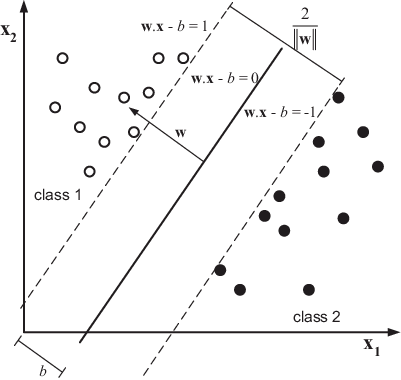
\includegraphics[scale=0.5]{SVM-separating-hyperplane}
\caption{Hyperplane separating two classes of input data \cite{SVMdiag}}
\end{figure}
Maximizing the margin of this hyperplane $\frac{2}{||w||}$ is computed by computing min$\frac{1}{2}||W||^2$, where $W = \sum_{i=1}^N \alpha_i^{*}x_iy_i$. Computation now only involves the minimizing of a quadratic function. For features that cannot be separated linearly, kernel functions which operate in higher dimensions can be used to classify the feature. 

Babu and Mohan \cite{SVM} use SVM to classify various three phase short circuit faults by first extracting event features with the Hilbert Huang Transform (HHT) which outputs instantaneous amplitude, phase and frequency. From the HHT, the following features were used to train a SVM for each of the three phases A, B \& C:
\begin{itemize}
\item Energy distribution of instantaneous amplitude 
\item Standard deviation of amplitude
\item Standard deviation of phase 
\end{itemize}
For each phase, SVM output 1 if there was a fault detected and -1 if there was no fault detected. Results are further defined in Table 5.
\begin{table}[H]
\centering
\begin{tabular}{|c|c|c|c|}
\hline
SVM A & SVM B & SVM C & Fault Type\\
\hline
\hline
\cellcolor{red!25}1 & -1 & -1 & Single Line (A) to Ground\\
\hline
-1 & \cellcolor{red!25}1 & -1 & Single Line (B) to Ground \\
\hline
-1 & -1 & \cellcolor{red!25}1 & Single Line (C) to Ground\\
\hline
\cellcolor{red!25}1 & \cellcolor{red!25}1 & -1 & Double Line (AB) to Ground\\
\hline
\cellcolor{red!25}1 & -1 & \cellcolor{red!25}1 & Double Line (AC) to Ground\\
\hline
-1 & \cellcolor{red!25}1 & \cellcolor{red!25}1 & Double Line (BC) to Ground  \\
\hline 
\cellcolor{red!25}1 & \cellcolor{red!25}1 &\cellcolor{red!25} 1 & Other\\
\hline
\end{tabular}
\caption{Fault Classification using SVM }
\end{table}

Babu and Mohan reported a 95.33\% accuracy efficiency from the results gathered. We note that this SVM method is only useful in detecting voltage sag and interruptions and not other PQ disturbances. However, this method does take into account all three phases and is able to successfully detect whether the fault is SLG or DLG and classify the fault, whereas other classification methods have not considered the classification of a particular voltage sag or interruption.


\newpage 
\section{Project Plan}
\subsection{Milestones}
The following tables outline deadline and objectives of major project milestones to be completed throughout the duration of this thesis project. Milestones in bold are ITEE Thesis Assessment Items. Note that all milestones up to and including Week 5 have been completed.
\begin{table}[H]
\begin{adjustwidth}{-.5in}{-.5in}  
\begin{center}
\begin{tabular}{|M{20mm}|>{\RaggedRight}p{0.25\textwidth}|>{\RaggedRight}p{0.65\textwidth}|}
\hline
Deadline & Milestone & Objective \& Notes\\
\hline
\multirow{2}{*}[-3mm]{Week 1} & Meet with Supervisor & Discuss project details and expectations\\
\cline{2-3}
& Begin Literature Review & Gather reputable sources and increase content knowledge\\
\hline
\multirow{2}{*}{Week 2} & \multirow{2}{*}{Receive Sample Data} & Become familiar with data arrangement and exportation\\
& & Determine best programming language to analyse data\\
\hline
\multirow{1}{*}[-6mm]{Week 4} & Choose literature to be reviewed in proposal & Determine the most relevant and successful algorithms to discuss in proposal\\
\hline
\multirow{1}{*}[-3mm]{Week 5} & \multirow{1}{*}[-3mm]{\textbf{Project Proposal}} & Complete Literature Review, Project Plan and summarise objectives and motivation of project\\
\hline
\multirow{1}{*}[-3mm]{Week 7} & Replicate at least one detection algorithm & Using MATLAB or Python on any test data and comment on efficiency and accuracy\\
\hline
\multirow{2}{*}[-6mm]{Week 8} & Replicate at least two detection algorithms & Using Python on any test data and comment on efficiency and accuracy\\
\cline{2-3}
& Progress meeting with supervisor & Discuss current results and update expectations on result accuracy\\
\hline
\multirow{1}{*}[-3mm]{Week 9} & Replicate at least 2 detection algorithms & Using Python on provided data\\
\hline
\multirow{3}{*}[-12mm]{Week 10} & Continue progress on detection algorithms & Gathering a summary and discussion of results in preparation for the seminar\\
\cline{2-3}
& Potential Classification Algorithm start & Attempt of classifying events in any language with any test or provided data\\
\cline{2-3}
& Format Seminar Presentation & Speech, Visuals (PPTX), Demonstrations\\
\hline
\multirow{2}{*}[-3mm]{Week 11} & \textbf{Progress Seminar} & Gather and present results from tested algorithms\\ 
\cline{2-3}
& \textbf{Seminar Attendance} & \\
\hline 
\end{tabular}
\end{center}
\end{adjustwidth}
\caption{Semester 1 objectives and deadlines}
\end{table}


\begin{table}[H]
\begin{adjustwidth}{-.5in}{-.5in}  
\begin{center}
\begin{tabular}{|M{20mm}|>{\RaggedRight}p{0.25\textwidth}|>{\RaggedRight}p{0.65\textwidth}|}
\hline
Deadline & Milestone & Objective \& Notes\\
\hline
\multirow{2}{*}[-3mm]{Week 2} & Progress Meeting with supervisor & Discuss progress after summer break and update expectations \\
\cline{2-3}
& Thesis Writing & Begin writing non-results based areas\\
\hline
\multirow{2}{*}[-6mm]{Week 4}& Determine most accurate detection algorithm & Journal and record results from previous tests of various algorithms for detection \\
\cline{2-3}
& Thesis Writing & Results from detection\\
\hline 
\multirow{2}{*}[-9mm]{Week 6} & Deploy detection algorithms & On provided data from aged transformer\\
\cline{2-3}
& Determine most accurate classification algorithm & Journal and record results from previous tests of various algorithms for classification\\
\hline 
\multirow{2}{*}[-3mm]{Week 9} & Deploy classification algorithms & On provided data from aged transformer\\
\cline{2-3}
& Thesis Writing & Results from classification\\
\hline
\multirow{2}{*}[-6mm]{Week 10} & Progress Meeting with supervisor & Discuss progress on project and discuss Thesis writing\\
\cline{2-3}
& Demonstration Preparation & Gather results and prepare presentation for demonstration\\
\hline 
\multirow{1}{*}[-3mm]{Week 12} & \textbf{Poster and Demonstration} & Gather and present results from project duration\\ 
\hline
SWOTVAC & \textbf{Thesis} & \\
\hline 
\end{tabular}
\end{center}
\end{adjustwidth}
\caption{Semester 2 objectives and deadlines}
\end{table}



\newpage
\subsection{Risk Assessment}

Table 9 summarises the potential non-OHS risks to the project:

\begin{table}[H]
\begin{adjustwidth}{-.5in}{-.5in}  
\begin{center}
\begin{tabular}{|>{\RaggedRight}p{0.6\textwidth}|>{\RaggedRight}p{0.3\textwidth}|>{\RaggedRight}p{0.2\textwidth}|}
\hline
Risk \& Impact on Project & Potential Cause \& Likelihood & Mitigation Strategy\\
\hline
\textbf{Data Loss} & &\\
A loss of data will be catastrophic to the project as this would completely halt any progress to the project. Algorithms would not be able to be deployed successfully.
&
\begin{itemize}
\item Corruption of data
\item Damage to hard drive
\item Misplacement or damage to computer
\end{itemize} 
&  Backing up data to multiple locations, including cloud \\
\underline{Impact: High} & \underline{Likelihood: Low} & \\
\hline
\textbf{Document File Loss} & &\\
Losing a document such as the Thesis file can result in a shortened timespan to complete if a high amount of progress has been made. As a result, the final report submitted may be of a lower quality due to a rush to complete. & \begin{itemize}
\item Corruption of file
\item Damage to hard drive
\item Misplacement of damage to computer
\item LaTeX files corrupted
\end{itemize} & Frequent saving and drafting of TeX files and using GIT for version control.\\
\underline{Impact: Medium} & \underline{Likelihood: Low} &\\
\hline
\textbf{Insufficient Time} & &\\
This project requires developing and deploying algorithms on large sets of data, which takes up a considerable amount of time. If milestones and the plan are not up-kept, it is possible that no feasible results are achieved. & \begin{itemize}
\item Poor time management
\item Assessment from other courses
\item Personal stresses 
\end{itemize} & 
Frequent meetings with supervisor to motivate progress. Personal initiative to complete tasks for the project.\\
\underline{Impact: Medium} & \underline{Likelihood: Medium} &\\
\hline
\textbf{Health Related Impacts} & &\\
Poor health will hinder the ability to complete the project. Furthermore, a lockdown may be imminent due to COVID-19. Although this project can be completed remotely, mental health risks may also affect quality of work. & \begin{itemize}
\item COVID-19 Virus
\item Other unexpected physical/mental issues
\end{itemize} & 
Following QLD Health advice and keeping a healthy work-life balance.\\
\underline{Impact: Low} & \underline{Likelihood: Medium} &\\
\hline

\end{tabular}
\end{center}
\end{adjustwidth}

\caption{Risk Assessment for Thesis Project}
\end{table}

\subsection{OHS Risk Assessment}
The majority of the work undertaken for this project will not be completed in a laboratory environment, so there is a low level of risk which is covered by general OHS rules. 

\newpage
\section{Bibliography}
\printbibliography[heading=none]

\end{document}
